% !TEX root = ../main.tex
\paragraph{High Threshold Cherenkov Counter (HTCC)}
\label{par::htcc}
    \begin{wrapfigure}{l}{0.50\textwidth}
        \centering\frame{
        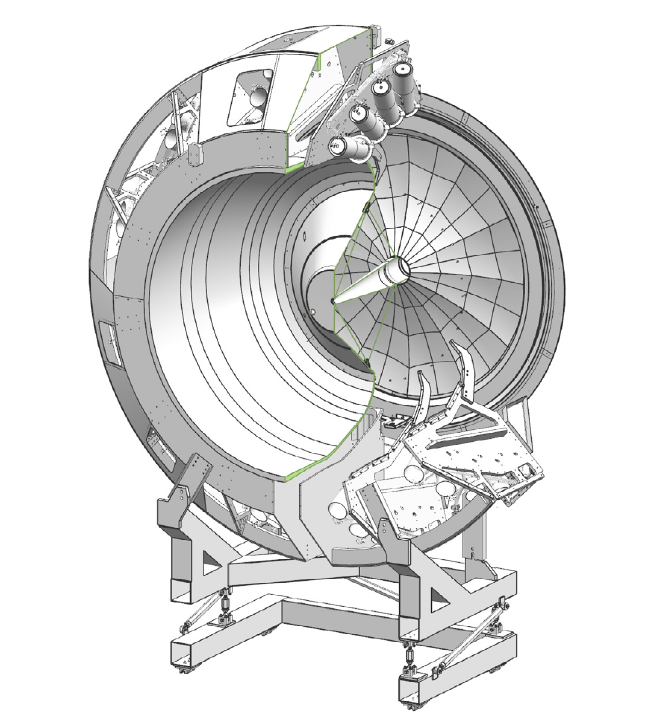
\includegraphics[width=\linewidth]{211htcc.png}}
        \caption[HTCC]{Render of the High Threshold Cherenkov Counter.
        The container spans a diameter of about 4.5 m. The mirror is seen at the downstream end to the right.
        The PMTs are mounted in 12 sectors and in groups of 4 at the outer perimeter of the container.
        Light collection uses additional Winston cones and 5-in PMTs with quartz windows.}
        \label{fig::htcc}
    \end{wrapfigure}

    The HTCC is the main detector to separate electrons and positrons with momenta below 4.9 GeV from other charged particles.
    The detector has full azimuthal coverage and spans from $5\degree$ to $35\degree$ in polar angle.
    It has no blind areas in its complete solid angle coverage.
    The detector is located downstream of the target, fitted in between magnets, upstream of the forward tracking detectors.

    The HTCC system is mainly used for electron/positron identification, and thus it provides high rejection of charged pions and low background noise for reliable identification of scattered electrons in a dense electromagnetic background environment.
    The HTCC is a single unit operated in dry CO2 gas at 1 atm pressure.
    It is constructed using a multi-focal mirror of 48 elliptical mirror facets that focuses the Cherenkov light on 48 PhotoMultiplier Tubes (PMTs), each with a quartz window of 125 mm diameter.
    The PMTs are located in a magnetic field of up to $3.5\cdot 10^{-3}$ T oriented along the phototube axes and are surrounded along their lengths by a multi-layer magnetic shield with active compensation coils.

    In order to minimize multiple scattering in the HTCC detector materials and to limit its impact on the momentum analysis of charged tracks in the torus field, the HTCC mirror system is constructed using a backing structure of low-density composite material.
    As the detector is located in front of the momentum analysing torus magnet, all materials but the radiator gas in the path of the charged particles had to be kept to a minimum.
    In the actual detector, the density of the solid material seen by charged particles passing through the HTCC volume is $135 ~\text{mg}/\text{cm}^2$.
    The HTCC is also used to generate a fast signal to be used as a trigger for scattered electrons.
    The HTCC operates in conjunction with energy deposited in the electromagnetic calorimeters to identify electrons of specific energies \cite{sharabian2020}.
    A cut view of HTCC can be seen in Figure \ref{fig::htcc}.
